\documentclass[aspectratio=169,14pt]{beamer}
\usepackage[utf8]{inputenc}
\usepackage[russian]{babel}
\usetheme{Madrid}
\usecolortheme{whale}

\title[ДЗ ИМ]{Домашнее задание}
\subtitle{Профиль: Прог}
\author{Никита Попов}
\date{23 апреля 2026 г.}

\setbeamertemplate{footline}{%
  \leavevmode%
  \hbox{%
    \begin{beamercolorbox}[wd=.33\paperwidth,ht=2.25ex,dp=1ex,center]{author in head/foot}%
      \usebeamerfont{author in head/foot}\insertshortauthor
    \end{beamercolorbox}%
    \begin{beamercolorbox}[wd=.33\paperwidth,ht=2.25ex,dp=1ex,center]{title in head/foot}%
      \usebeamerfont{title in head/foot}\insertshorttitle
    \end{beamercolorbox}%
    \begin{beamercolorbox}[wd=.34\paperwidth,ht=2.25ex,dp=1ex,right]{date in head/foot}%
      \usebeamerfont{date in head/foot}\insertshortdate{}\hspace*{2em}
      \insertframenumber{} / \inserttotalframenumber\hspace*{2ex}
    \end{beamercolorbox}}%
  \vskip0pt%
}
\setbeamertemplate{navigation symbols}{}

\usepackage{graphicx}
\usepackage{booktabs}
\usepackage{tikz}

\begin{document}

\begin{frame}[plain]
  \titlepage
\end{frame}

\begin{frame}{Содержание}
  \tableofcontents
\end{frame}

\section{Задание 1: Товары и валюты}

\begin{frame}{Товары из Японии}
  \textbf{Страна:} Япония (унитарная монархия)
  \vspace{0.3cm}

  \begin{columns}[T]
    \column{0.3\textwidth}
      \textbf{Toyota Camry}
      \begin{itemize}
        \item Цена: 3\,500\,000 ¥
        \item 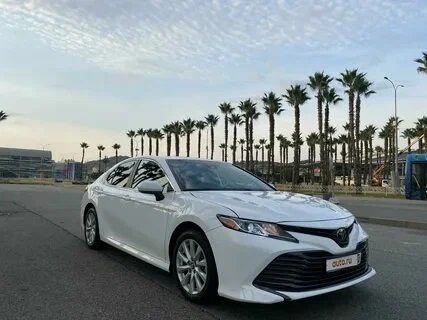
\includegraphics[width=\linewidth]{camry.jpg}
      \end{itemize}
    \column{0.3\textwidth}
      \textbf{Sony PS5}
      \begin{itemize}
        \item Цена: 60\,000 ¥
        \item 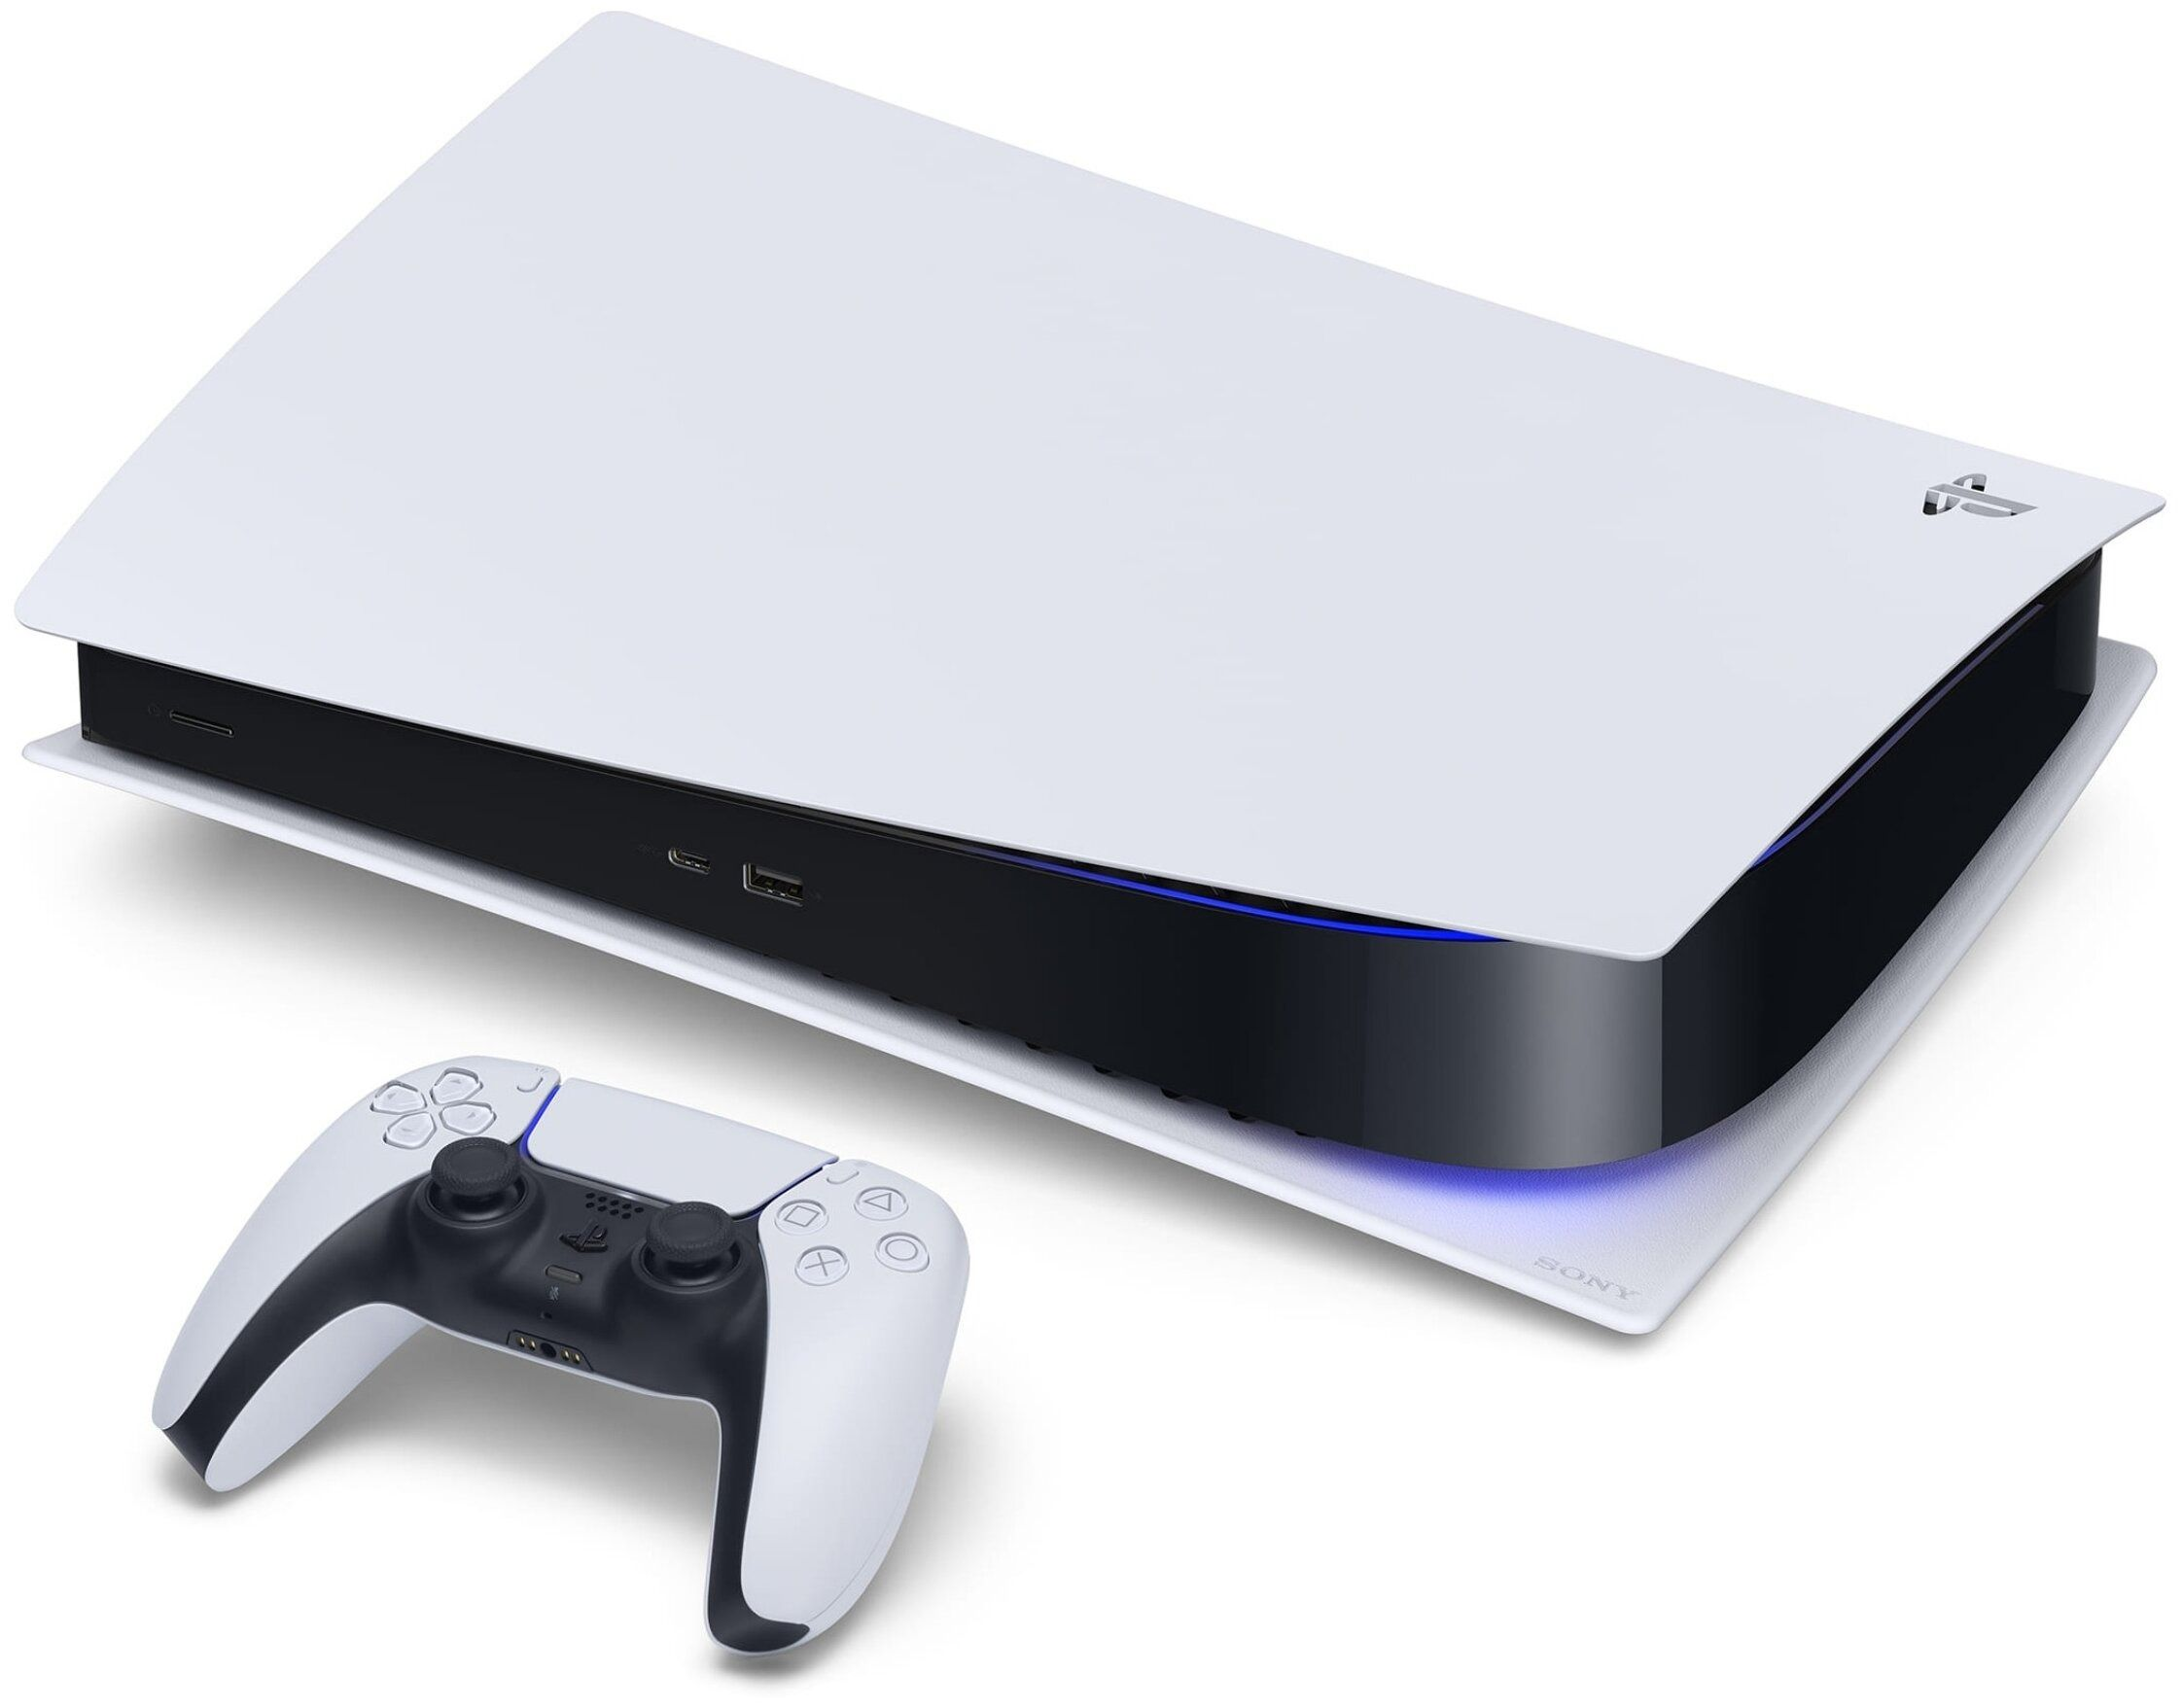
\includegraphics[width=\linewidth]{ps5.jpg}
      \end{itemize}
    \column{0.3\textwidth}
      \textbf{Nintendo Switch}
      \begin{itemize}
        \item Цена: 35\,000 ¥
        \item 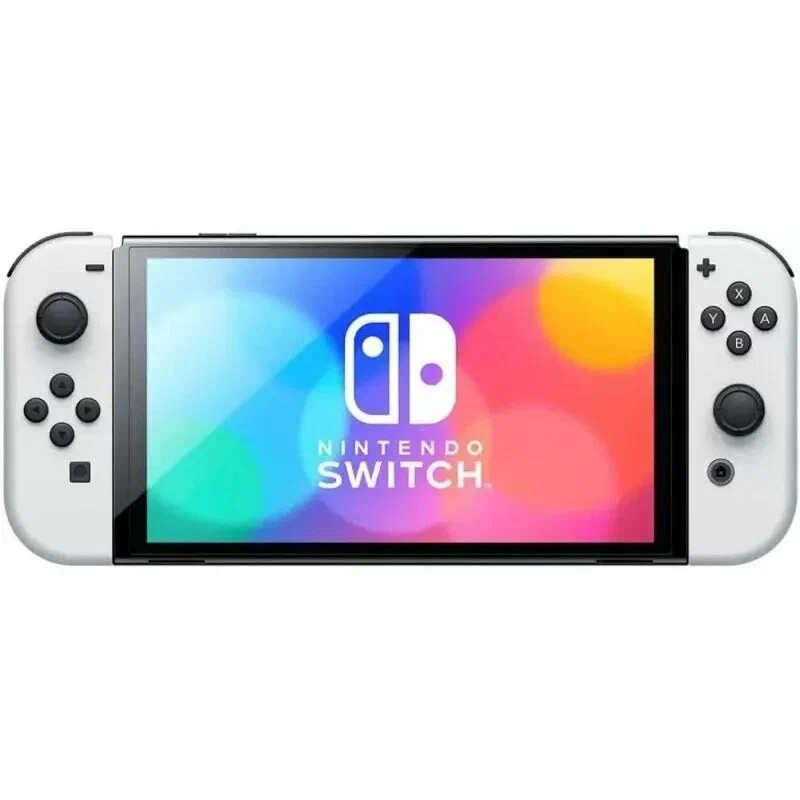
\includegraphics[width=\linewidth]{switch.jpg}
      \end{itemize}
  \end{columns}
\end{frame}

\begin{frame}{Стоимость в грузинских лари и евро}
  \small
  Курсы валют: 1 ¥ = 0.0171 GEL; 1 ¥ = 0.0062 EUR.
  \vspace{0.2cm}

  \begin{columns}[T]
    \column{0.65\textwidth}
      \begin{table}[h]
        \footnotesize
        \centering
        \begin{tabular}{lrrr}
          \toprule
          Товар & Цена (¥) & Цена (GEL) & Цена (€) \\
          \midrule
          Toyota Camry & 3\,500\,000 & 59\,850 & 21\,700 \\
          Sony PS5 & 60\,000 & 1\,026 & 372 \\
          Nintendo Switch & 35\,000 & 599 & 217 \\
          \midrule
          \textbf{Итого} & \textbf{3\,595\,000} & \textbf{61\,475} & \textbf{22\,289} \\
          \bottomrule
        \end{tabular}
      \end{table}
    \column{0.35\textwidth}
      \hfill
      \begin{tabular}{c}
        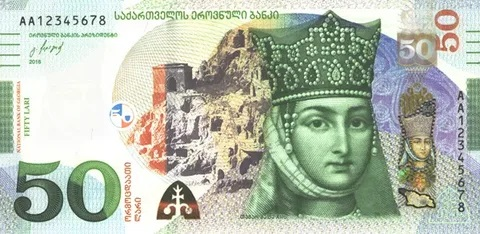
\includegraphics[height=2cm]{lari.jpg} \\
        Грузинский лари (GEL) \\[0.4cm]
        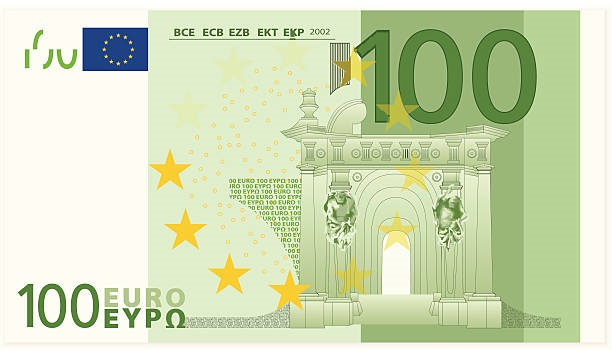
\includegraphics[height=2cm]{euro.jpg} \\
        Евро (EUR)
      \end{tabular}
      \hspace{0.2cm}
  \end{columns}
\end{frame}

\section{Задание 2: Криптовалюты}

\begin{frame}{Плюсы и минусы криптовалют}
  \begin{block}{Основная валюта}
    Децентрализованные цифровые деньги вместо фиата.
  \end{block}

  \begin{columns}[T]
    \column{0.5\textwidth}
      \textbf{Плюсы}
      \begin{itemize}
        \item Децентрализация
        \item Низкие комиссии
        \item Прозрачность
        \item Ограниченная эмиссия
        \item Доступ без банков
      \end{itemize}
    \column{0.5\textwidth}
      \textbf{Минусы}
      \begin{itemize}
        \item Волатильность
        \item Сложность регулирования
        \item Риск нелегальных операций
        \item Технические барьеры
        \item Необратимость ошибок
      \end{itemize}
  \end{columns}
\end{frame}

\section{Задание 3: Аэропорты}

\begin{frame}{Определение аэропортов}
  \begin{itemize}
    \item \textbf{KUF} – Курумоч, Самара, Россия
    \item \textbf{BKK} – Суварнабхуми, Бангкок, Таиланд
    \item \textbf{ATL} – Хартсфилд-Джексон, Атланта, США
  \end{itemize}
  \vspace{0.2cm}
  \begin{columns}[T]
    \column{0.33\textwidth}
      \centering
      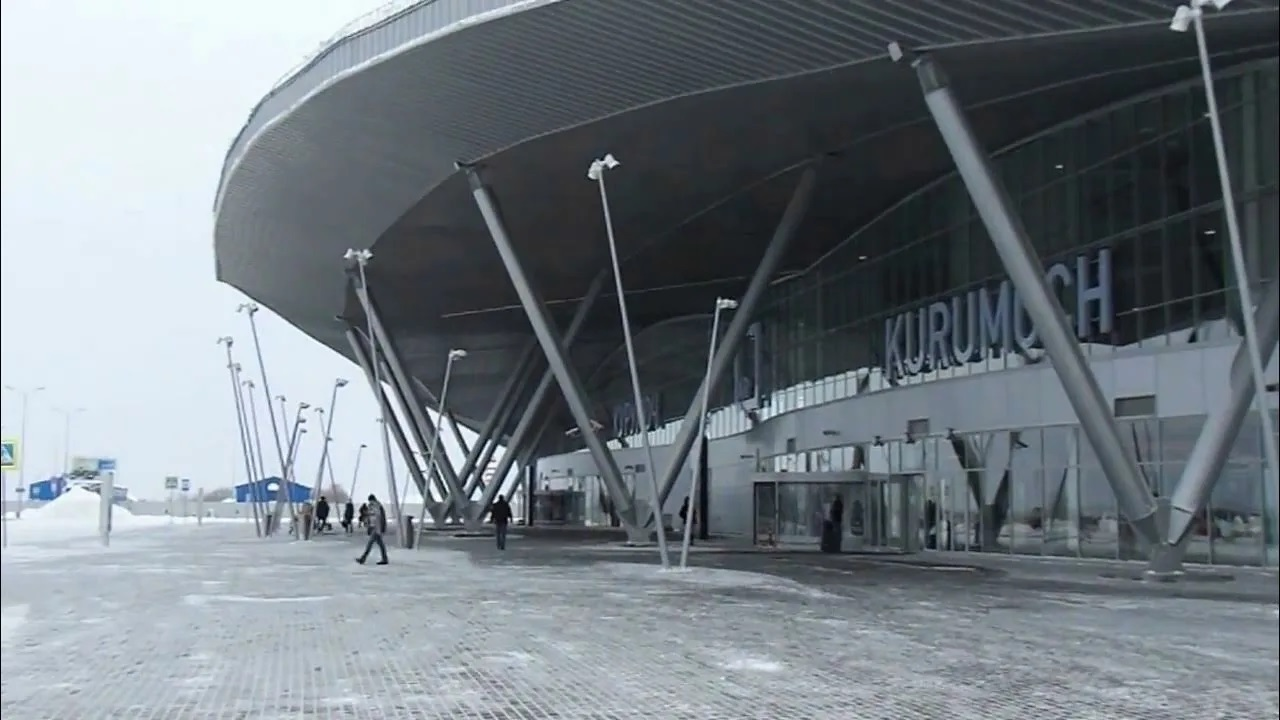
\includegraphics[height=2.5cm]{kuf.jpg}\\
      {\tiny Курумоч (KUF)}
    \column{0.33\textwidth}
      \centering
      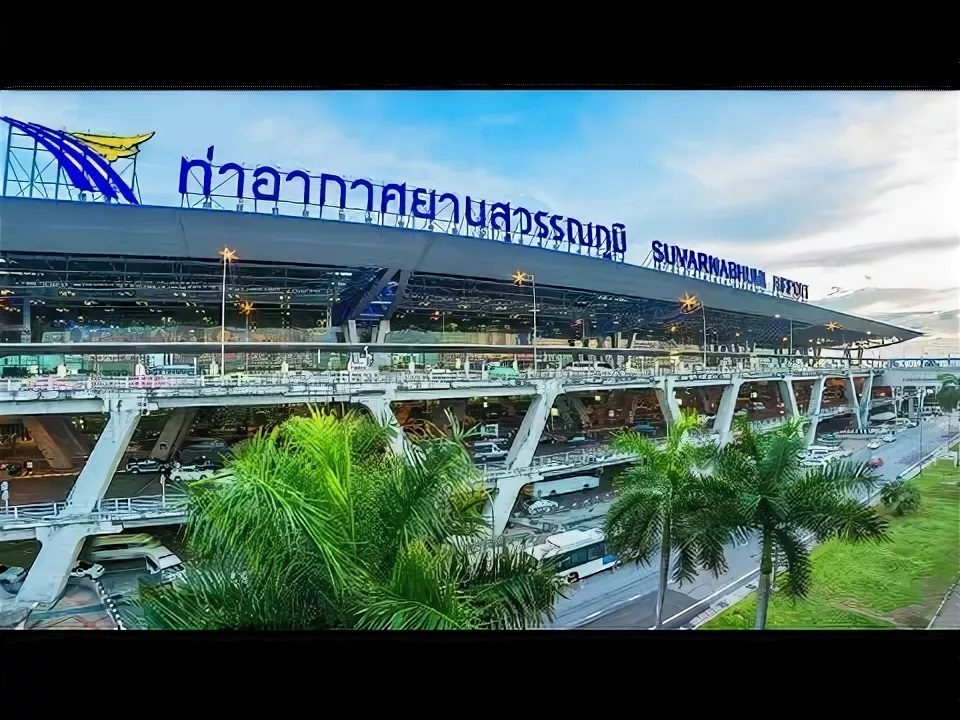
\includegraphics[height=2.5cm]{bkk.jpg}\\
      {\tiny Суварнабхуми (BKK)}
    \column{0.33\textwidth}
      \centering
      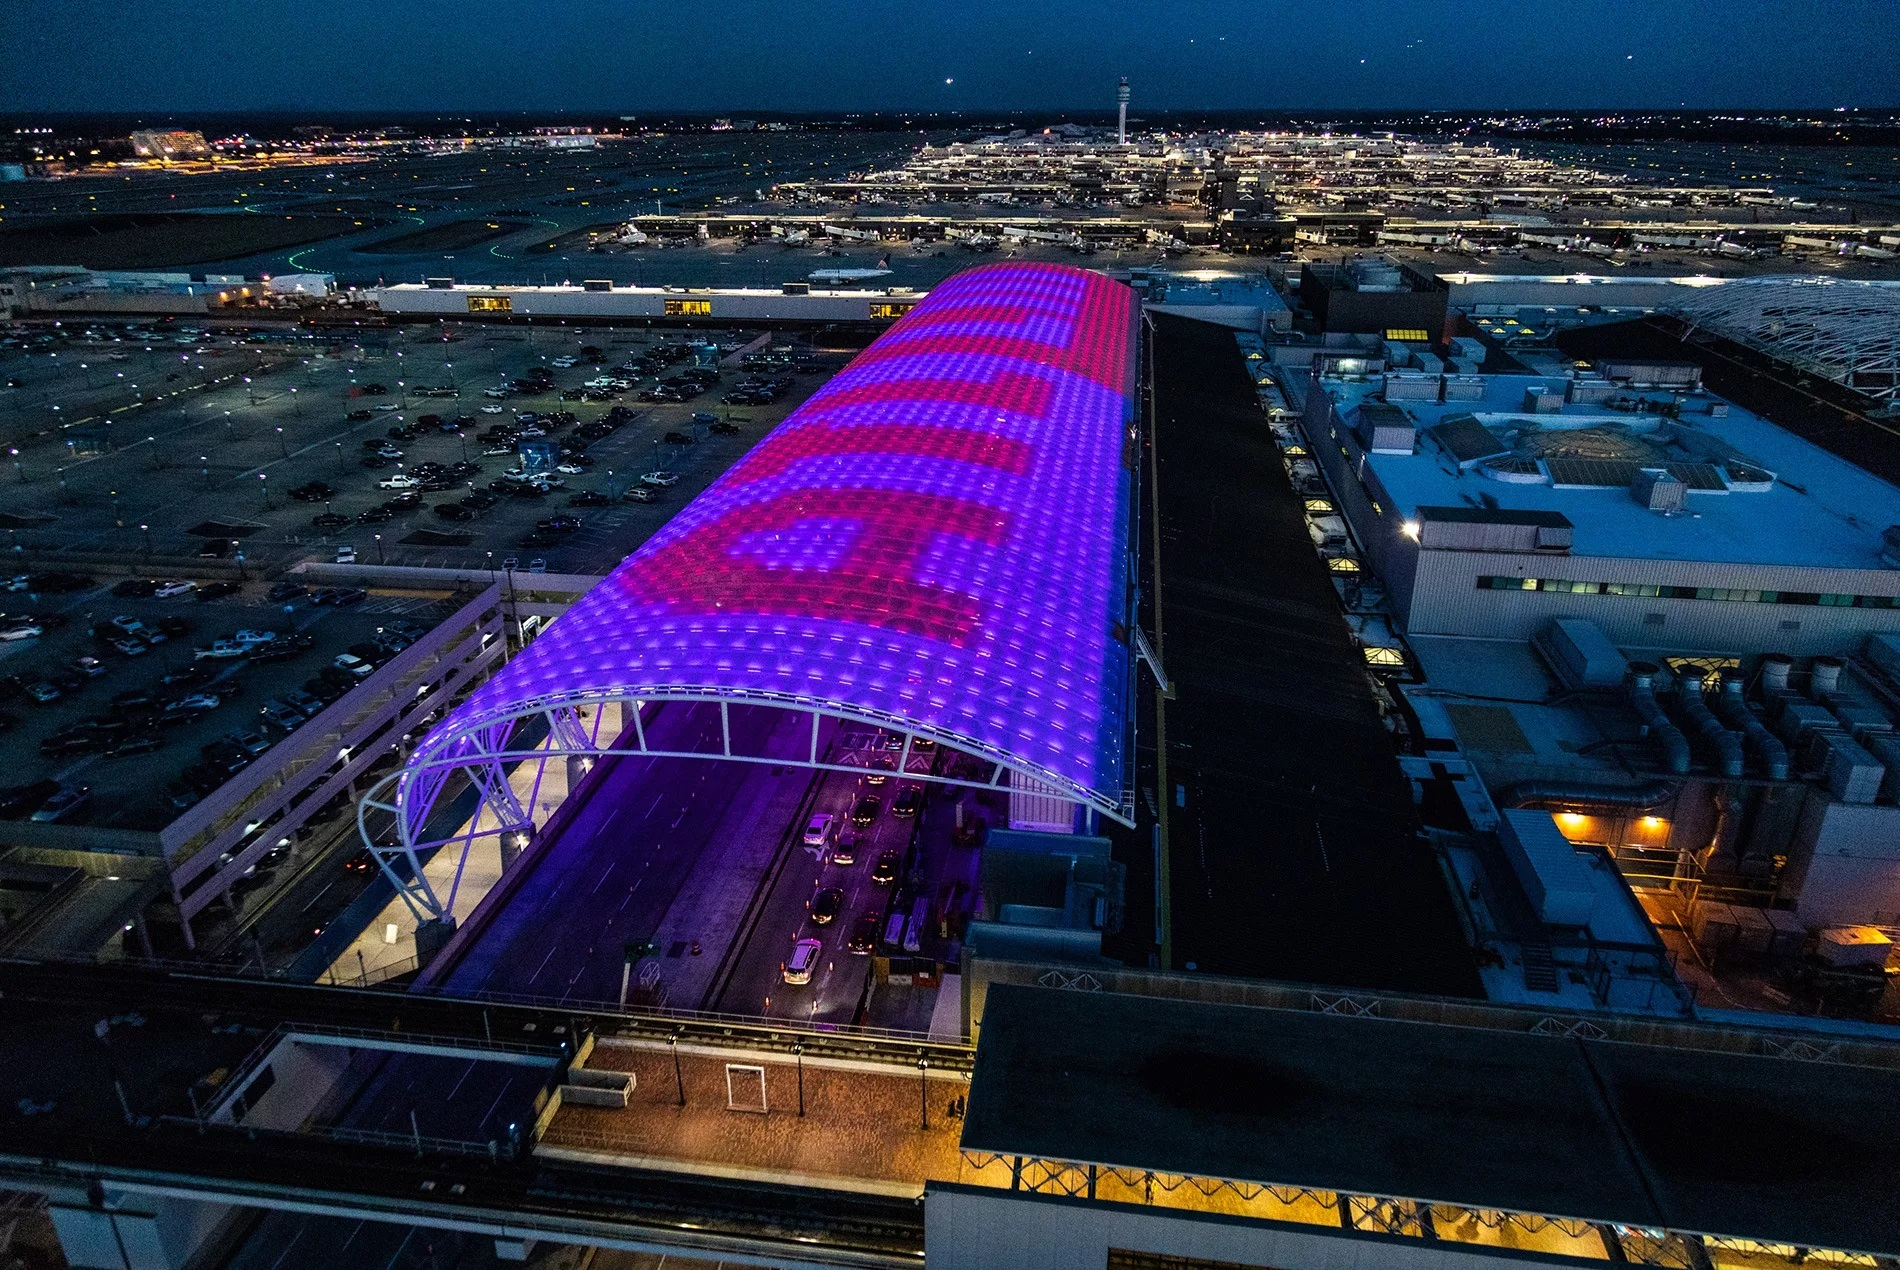
\includegraphics[height=2.5cm]{atl.jpg}\\
      {\tiny Хартсфилд-Джексон (ATL)}
  \end{columns}
\end{frame}

\begin{frame}{Статистика аэропортов}
  \begin{table}
    \centering
    \begin{tabular}{lccc}
      \toprule
      Параметр & KUF & BKK & ATL \\
      \midrule
      Вылетов в день & 34 & 484 & $\approx$ 1000 \\
      Направлений & 37 & 151 & 215 \\
      Стран & 11 & 47 & $> 70$ \\
      Популярный рейс & Москва & Пхукет (HKT) & Орландо (MCO) \\
      \bottomrule
    \end{tabular}
    Данные с Flightradar24
  \end{table}
\end{frame}

\section{Задание 4: Вылеты за час}

\begin{frame}{Количество вылетов за час}
  \begin{table}
    \centering
    \begin{tabular}{lccr}
      \toprule
      Аэропорт & Период & Рейсов & В среднем за час \\
      \midrule
      KUF & 5 часов & 7 & 1.4 \\
      BKK & 1 час & 21 & 21 \\
      ATL & 1 час & 48 & 48 \\
      \bottomrule
    \end{tabular}
  \end{table}
\end{frame}

\section{Задание 5: Сайт авиакомпании}

\begin{frame}{Макет сайта авиакомпании}
  \begin{center}
    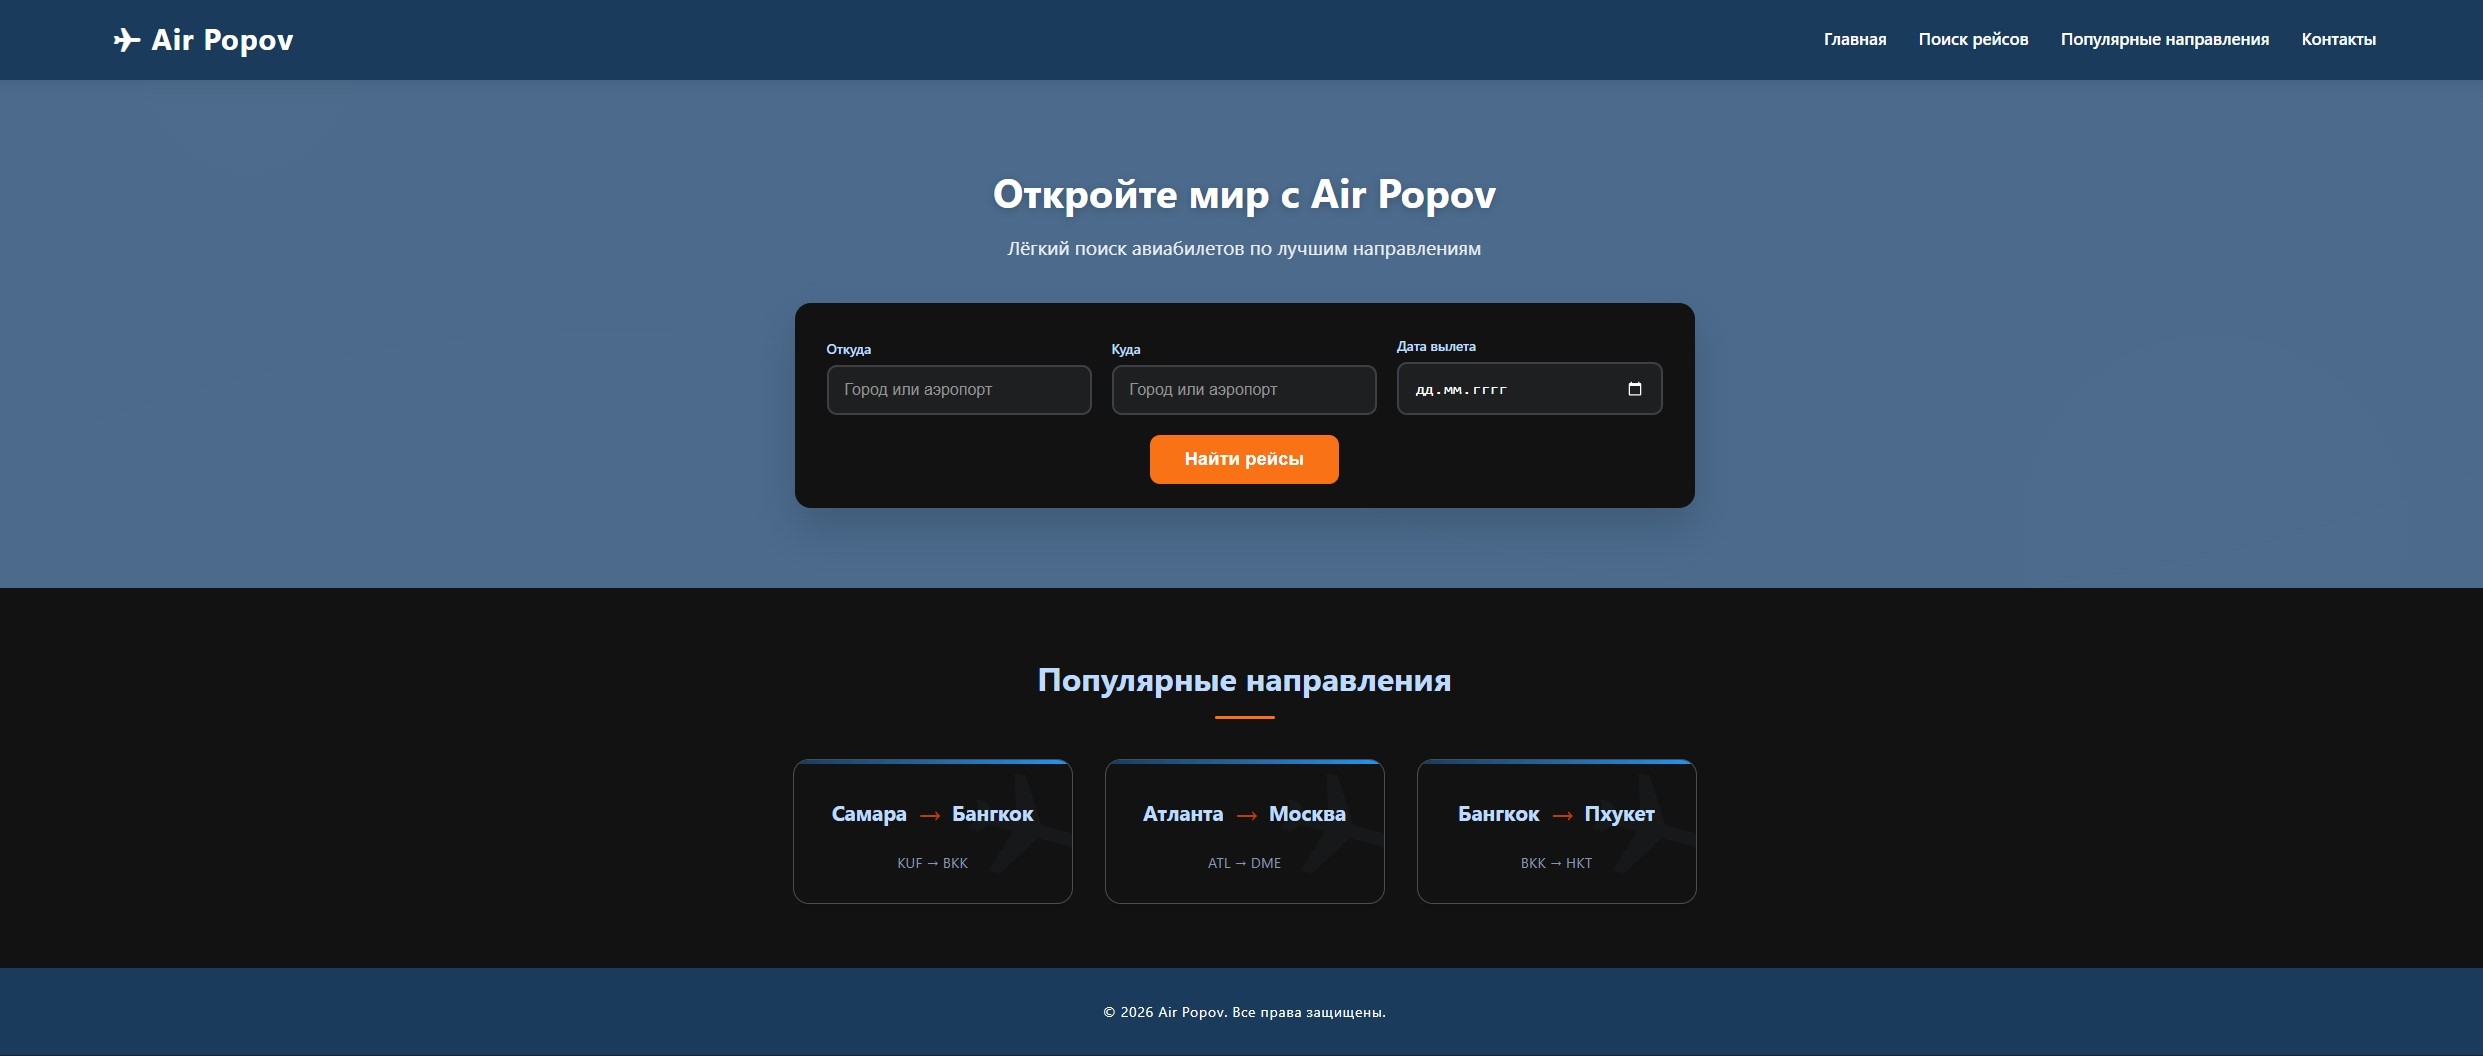
\includegraphics[width=\linewidth]{website.jpg}
  \end{center}
\end{frame}
\end{document}